\chapter{Prometheus and Grafana Monitoring Setup \\
\small{\textit{-- Annanya Jain, Luo Xu, Gavin Lam}
\index{Overleaf} 
\index{Chapter!PrometheusGrafana}
\label{Chapter::Prometheus and Grafana Monitoring Setup}}}

\section{Introduction}

This chapter documents our setup and configuration of a monitoring stack using \textbf{Prometheus}, \textbf{Grafana}, and \textbf{Node Exporter}. The objective was to collect, visualize, and analyze system-level metrics such as CPU usage, memory utilization, disk I/O, and network performance. 

\begin{center}
  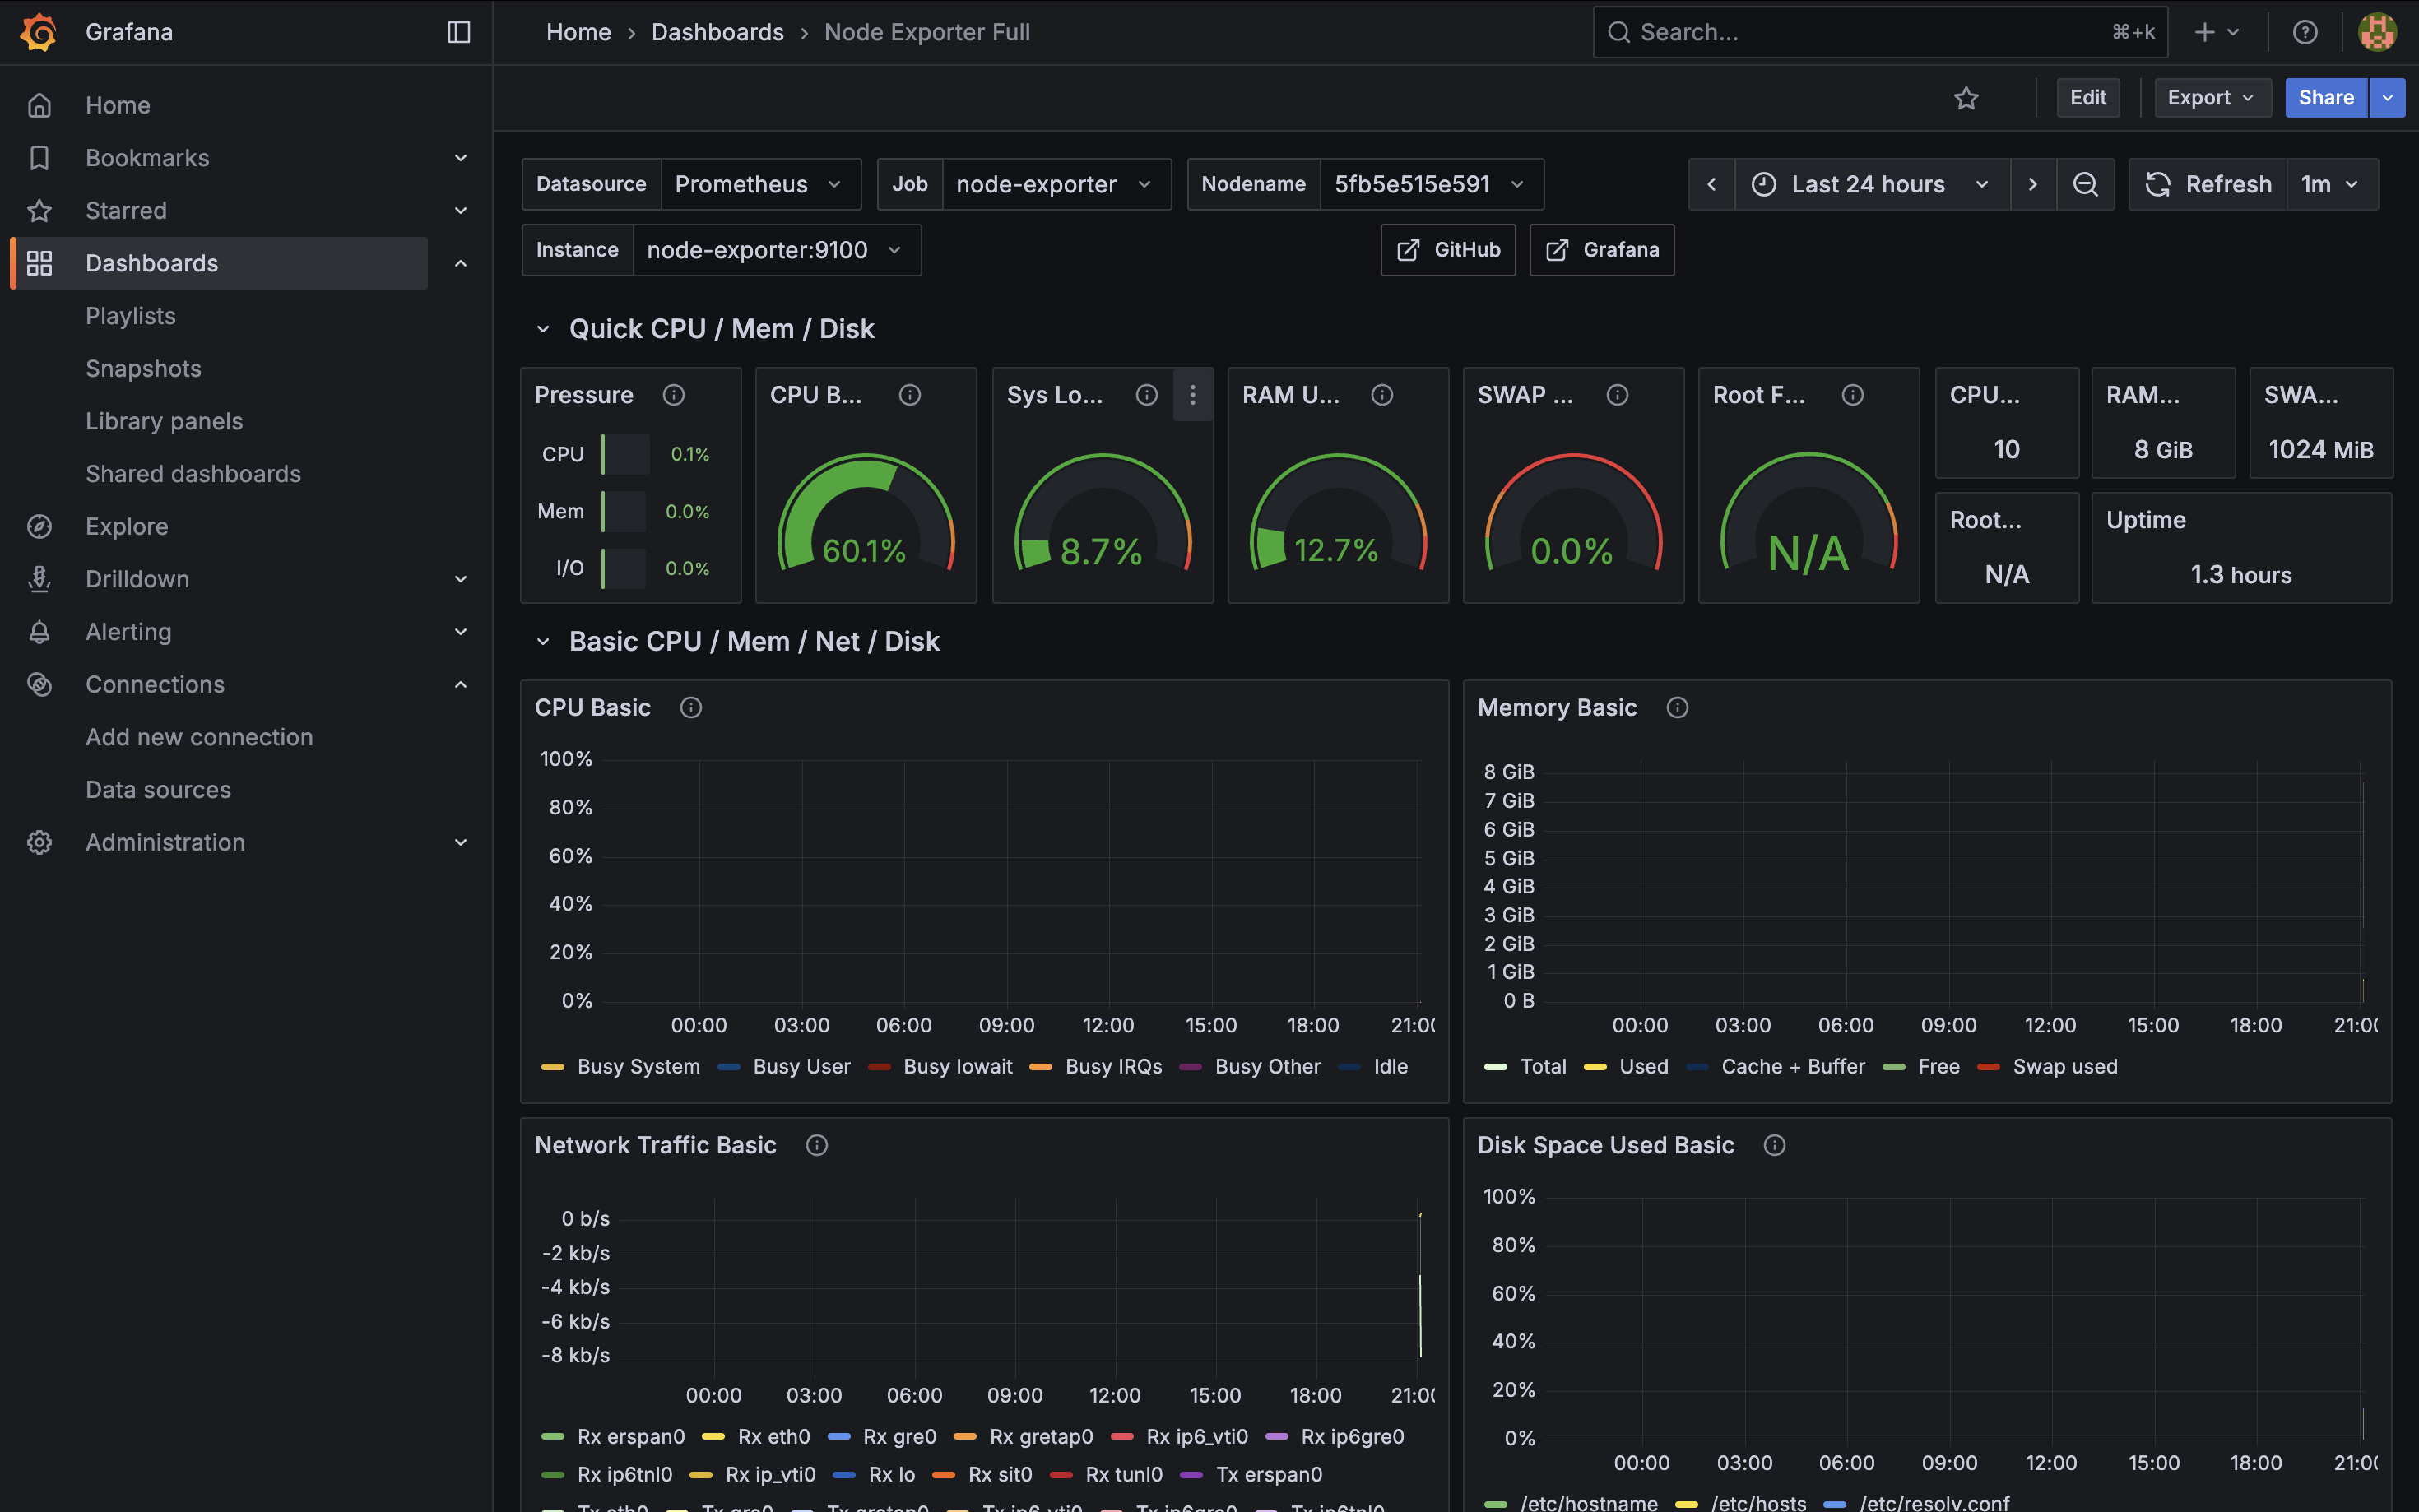
\includegraphics[width=0.9\textwidth]{png/Grafana.png}
\end{center}

\begin{center}
  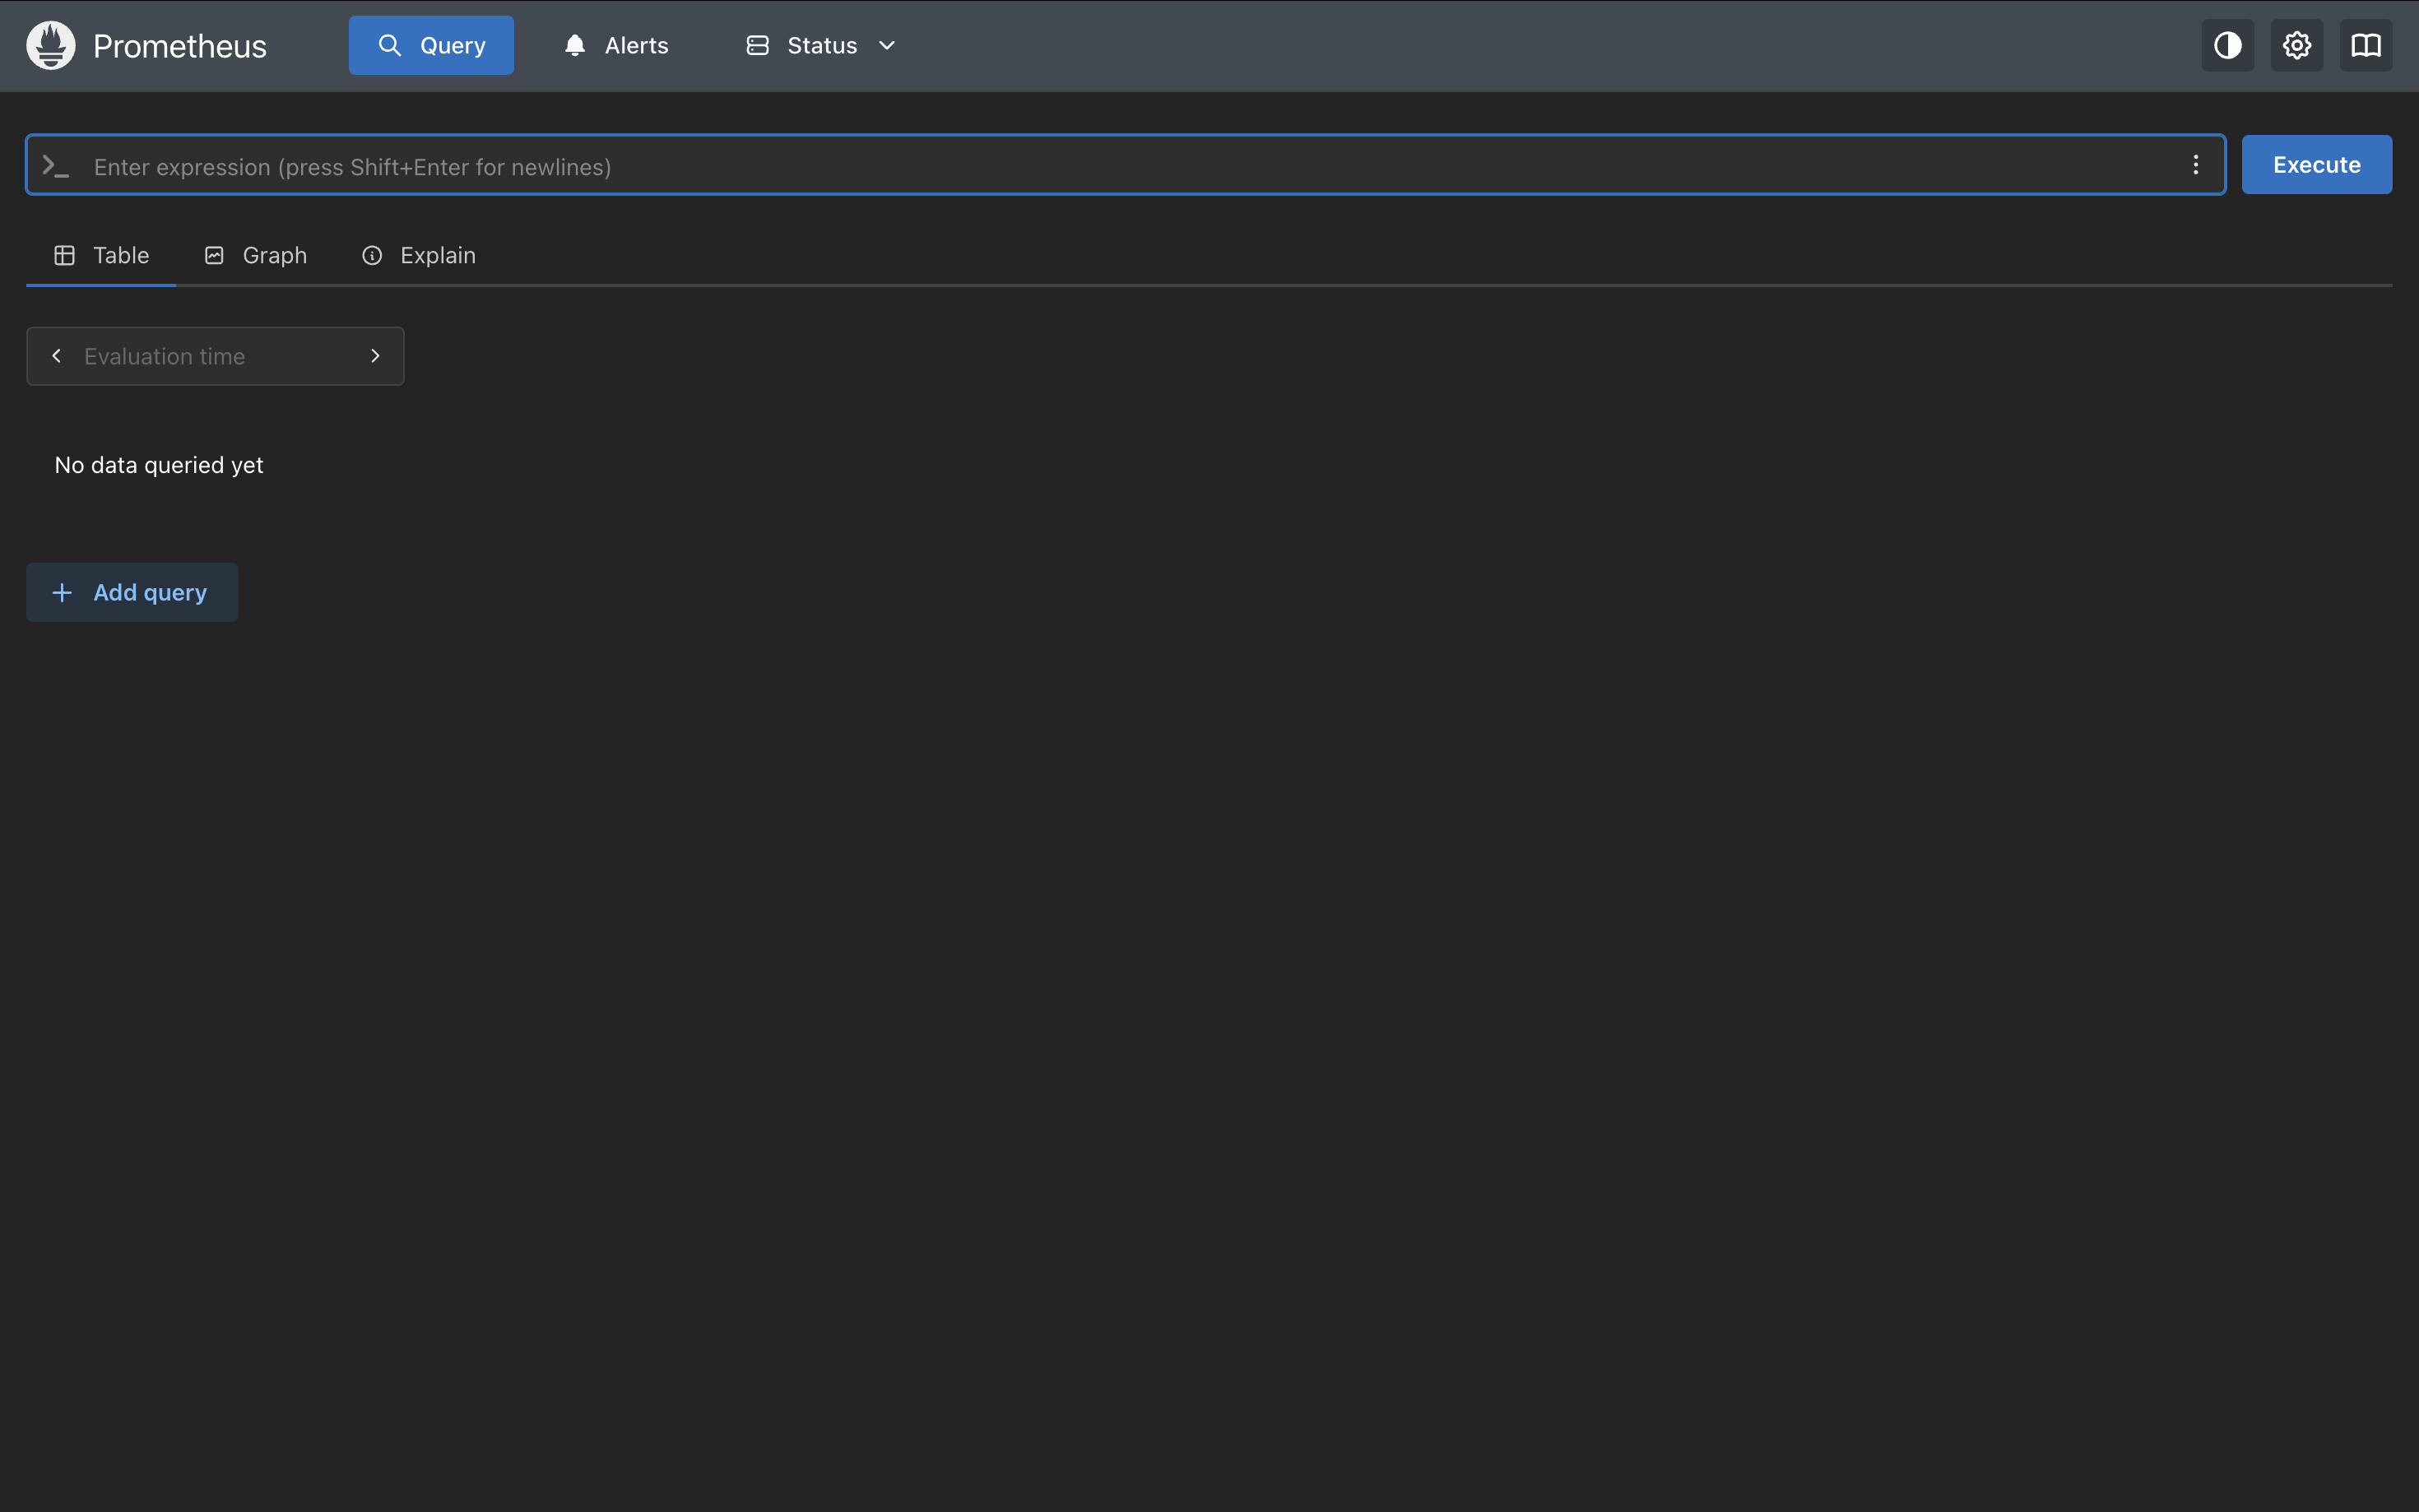
\includegraphics[width=0.9\textwidth]{png/Prometheus.png}
\end{center}


\section{The role of Prometheus, Grafana, and Node Exporter}
Prometheus is an open-source monitoring system that collects and stores time-series data from different sources, such as servers and applications. Node Exporter provides Prometheus with detailed system-level metrics like CPU usage, memory consumption, disk activity, and network performance. The Grafana dashboard visualizes key system health metrics collected by \textbf{Node Exporter} and stored by \textbf{Prometheus}. It provides a real-time overview of CPU, memory, disk, and network performance, allowing quick assessment of system status. \\

\textbf{What Dashboard 1860 tells you about system health?}

The top row displays a summary of \textbf{CPU}, \textbf{Memory}, and \textbf{Disk} utilization. In the captured dashboard, CPU usage is approximately \textbf{60\%}, memory usage around \textbf{12.7\%}, and swap usage is \textbf{0\%}, indicating stable performance with no significant resource pressure. Additional panels show detailed metrics:
\begin{itemize}
    \item \textbf{CPU Basic:} Tracks CPU activity over time and highlights user, system, and idle states.
    \item \textbf{Memory Basic:} Displays total, used, and free memory to detect potential memory issues.
    \item \textbf{Network Traffic:} Monitors data transmitted and received per network interface.
    \item \textbf{Disk Space Used:} Shows disk utilization across mounted file systems.
    \item \textbf{System Uptime:} Indicates total runtime of the node (about 1.3 hours in this case).
\end{itemize}

Overall, this dashboard provides an effective visualization of system performance and helps identify resource bottlenecks or irregular activity.

\section{Project Structure}
The following directory structure was used to organize configuration files and Docker services:

\begin{minted}[fontsize=\small,breaklines]{text}
PrometheusGrafana/
│
├── docker-compose.yml
├── prometheus/
│   ├── prometheus.yml
│   └── rules.yml
└── grafana/
    └── provisioning/
        └── datasources/
            └── datasource.yml
\end{minted}

\section{Docker Compose Configuration}
The monitoring stack consisted of three services: \textbf{Prometheus}, \textbf{Grafana}, and \textbf{Node Exporter}. 
These were defined in \texttt{docker-compose.yml} as follows:

\begin{minted}[fontsize=\small,breaklines]{yaml}
version: '3.8'

services:
  prometheus:
    image: prom/prometheus:latest
    container_name: prometheus
    volumes:
      - ./prometheus/prometheus.yml:/etc/prometheus/prometheus.yml
      - ./prometheus/rules.yml:/etc/prometheus/rules.yml
    ports:
      - "9091:9090"

  grafana:
    image: grafana/grafana:latest
    container_name: grafana
    ports:
      - "3000:3000"
    volumes:
      - ./grafana/provisioning:/etc/grafana/provisioning
    environment:
      - GF_SECURITY_ADMIN_USER=admin
      - GF_SECURITY_ADMIN_PASSWORD=admin
    depends_on:
      - prometheus

  node-exporter:
    image: prom/node-exporter:latest
    container_name: node-exporter
    ports:
      - "9100:9100"
\end{minted}

\noindent
In this configuration:
\begin{itemize}
    \item Prometheus runs on port \texttt{9091} (mapped from container port \texttt{9090}).
    \item Grafana runs on port \texttt{3000}.
    \item Node Exporter exposes system metrics on port \texttt{9100}.
\end{itemize}

\section{Prometheus Configuration}
The \texttt{prometheus.yml} file defines global settings, scrape intervals, and targets for metric collection:

\begin{minted}[fontsize=\small,breaklines]{yaml}
global:
  scrape_interval: 15s

rule_files:
  - "rules.yml"

scrape_configs:
  - job_name: 'prometheus'
    static_configs:
      - targets: ['localhost:9090']

  - job_name: 'node-exporter'
    static_configs:
      - targets: ['node-exporter:9100']
\end{minted}

\noindent
This configuration instructs Prometheus to:
\begin{itemize}
    \item Collect data every 15 seconds.
    \item Scrape metrics from itself on \texttt{localhost:9090}.
    \item Scrape metrics from Node Exporter at \texttt{node-exporter:9100}.
\end{itemize}

\section{Alerting Rules}
A rules file named \texttt{rules.yml} was created to define alerting conditions. 
This also resolved an earlier configuration error when Prometheus tried to load an empty directory as a rule file.

\begin{minted}[fontsize=\small,breaklines]{yaml}
groups:
  - name: example
    rules:
      - alert: InstanceDown
        expr: up == 0
        for: 1m
        labels:
          severity: critical
        annotations:
          summary: "Instance {{ $labels.instance }} down"
\end{minted}

\noindent
This rule triggers an alert if any monitored instance is down for more than one minute.

\section{Grafana Data Source Configuration}
Grafana was configured to use Prometheus as its default data source using the following file:  
\texttt{grafana/provisioning/datasources/datasource.yml}

\begin{minted}[fontsize=\small,breaklines]{yaml}
apiVersion: 1
datasources:
  - name: Prometheus
    type: prometheus
    access: proxy
    url: http://prometheus:9091
    isDefault: true
\end{minted}

\section{Launching the Monitoring Stack}
The monitoring setup was launched using Docker Compose:

\begin{minted}[fontsize=\small,breaklines]{bash}
docker compose up -d
\end{minted}

Once the containers were running, the following endpoints were verified:
\begin{itemize}
    \item Prometheus: \url{http://localhost:9091}
    \item Grafana: \url{http://localhost:3000}
    \item Node Exporter: \url{http://localhost:9100}
\end{itemize}

\section{Grafana Dashboard Setup}
After logging into Grafana using the default credentials (\texttt{admin/admin}), the \textbf{Node Exporter Full Dashboard (ID 1860)} was imported:

\begin{enumerate}
    \item Go to \texttt{+ → Import}.
    \item Enter Dashboard ID \texttt{1860} and click \texttt{Load}.
    \item Select \texttt{Prometheus} as the data source.
    \item Click \texttt{Import}.
\end{enumerate}

Auto-refresh was set to 10 seconds, and the time range was configured to display the last 5 minutes.

\section{Outcome and Observations}
After adding the rule file and restarting the containers, Prometheus began successfully scraping data from Node Exporter. The Grafana dashboard displayed real-time metrics such as:

\begin{itemize}
    \item CPU usage and load averages
    \item Memory and swap utilization
    \item Disk I/O statistics
    \item Network traffic rates
\end{itemize}

The system provided clear visibility into server performance and resource utilization.